\documentclass[12pt]{article}
\usepackage{graphicx}
\usepackage{listings}
\usepackage{xcolor}
\usepackage{circuitikz}

\graphicspath{ {./fig/} }

\definecolor{codegreen}{rgb}{0,0.6,0}
\definecolor{codegray}{rgb}{0.5,0.5,0.5}
\definecolor{codepurple}{rgb}{0.58,0,0.82}
\definecolor{backcolour}{rgb}{0.95,0.95,0.92}


\lstdefinelanguage{SPICE}{
  keywords={tran,ac,dc,subckt,meas,plot,print,control,run,end,endc, hardcopy},
  morecomment=[l]{*},
  morecomment=[l]{\$},
  morecomment=[s]{/*}{*/},
  morestring=[b]',
  morestring=[b]",
  ndkeywords={r,r1,r2,r3,r4,r5,l,l1,l2,l3,l4,l5,c,c1,c2,c3,c4,c5,v,vin,m,m1,m2,m3,m4,m5,d,d1,d2,d3,d4,d5,vdb, pulse,sin,i,pwl,exp},
  keywordstyle=\color{blue}\bfseries,
  ndkeywordstyle=\color{codegreen}\bfseries,
  identifierstyle=\color{black},
  commentstyle=\color{purple}\ttfamily,
  stringstyle=\color{red}\ttfamily,
  sensitive=true
}

\lstdefinestyle{mystyle}{
	backgroundcolor=\color{backcolour},   
    commentstyle=\color{codegreen},
    keywordstyle=\color{magenta},
    numberstyle=\tiny\color{codegray},
    stringstyle=\color{codepurple},
    basicstyle=\ttfamily\footnotesize,
    breakatwhitespace=false,         
    breaklines=true,                 
    captionpos=b,                    
    keepspaces=true,                 
    numbers=left,                    
    numbersep=5pt,                  
    showspaces=false,                
    showstringspaces=false,
    showtabs=false,                  
    tabsize=4
}

\lstset{style=mystyle}


% Title[Enter title of the experiment here]
\title{EE230: Homework-2\\
Unregulated DC Power Supply}

% Author[Enter details of author here]
\author{Prateek Garg, 20D070060}

% begin the document.
\begin{document}
\noindent
% make a title page.[this creates title page]
\maketitle

\section{Overview of the experiment} %[This segment creates Section as seen in document]

\subsection{Aim of the experiment}%[This segment creates sebsections under the same section]
\begin{enumerate}
	\item Understanding the problems associated with increasing the capacitor value in an unregulated powersupply so as to reduce the ripple.
  \item Understanding the limits of performance of a Zener regulator
  \item Understanding a BJT based series voltage regulator to appreciate the basic blocks of an IC voltage regulator.
\end{enumerate}


\subsection{Methods}

We start by creating a netlist for each circuit, simulating on Ngspice and exporting the values to a python script to plot them using Matplotlib.
\section{Design}
%Add circuit Diagrams here
%With accompaying Explanantions 
%<<<<<<< HEAD
% XCircuit output "RC_Integrator.eps.tex" for LaTeX input from RC_Integrator.eps.ps
\def\putbox#1#2#3{\makebox[0in][l]{\makebox[#1][l]{}\raisebox{\baselineskip}[0in][0in]{\raisebox{#2}[0in][0in]{#3}}}}
\def\rightbox#1{\makebox[0in][r]{#1}}
\def\centbox#1{\makebox[0in]{#1}}
\def\topbox#1{\raisebox{-\baselineskip}[0in][0in]{#1}}
\def\midbox#1{\raisebox{-0.5\baselineskip}[0in][0in]{#1}}
\begin{flushleft}
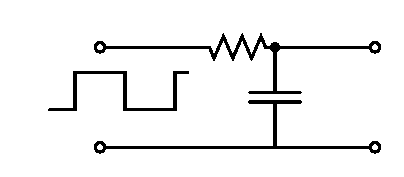
\includegraphics[width=\textwidth]{RC_Integrator.eps}\\
% translate x=624 y=118 scale 0.38
\putbox{1.31in}{0.84in}{R=10K$\Omega$}%
\putbox{1.81in}{0.25in}{C=0.1$\mu$F}%
\putbox{0.06in}{0.42in}{$V_{in}$}%
\putbox{0.47in}{0.50in}{5v}%
\putbox{0.89in}{0.25in}{0v}%
\end{flushleft}
=======
\begin{center}
    \begin{circuitikz}[american voltages]
        \draw
        (0,0) to [short, o-o] (6,0)
        to [open, v>=$V_{out}$] (6,4) 
        (0,0) to [open, v^>=$V_{in}$,o-o] (0,4)  
        to [R, l= $10K \Omega $,o-o] (6,4)
        (5,4) to [C, l_=$0.1\mu F$,*-*] (5,0); 
    \end{circuitikz}

    RC Integrator Circuit
\end{center}

>>>>>>> circuitikz

%\begin{center}
    \begin{circuitikz}[american voltages]
        \draw
        (0,0) to [short, o-o] (6,0)
        to [open, v>=$V_{out}$] (6,4) 
        (0,0) to [open, v^>=$V_{in}$,o-o] (0,4)  
        to [C, l_=$0.1\mu F$,o-o] (6,4)
        (5,0) to [R, l= $10K \Omega $,*-*] (5,4); 
    \end{circuitikz}

    RC Differentiator Circuit
\end{center}



\section{Simulation results}

\subsection{RC Integrator}
\subsubsection{Code snippet}
\lstinputlisting[language=SPICE]{../RC_Integrator.cir}
\subsubsection{Simulation results}
\makebox[\textwidth]{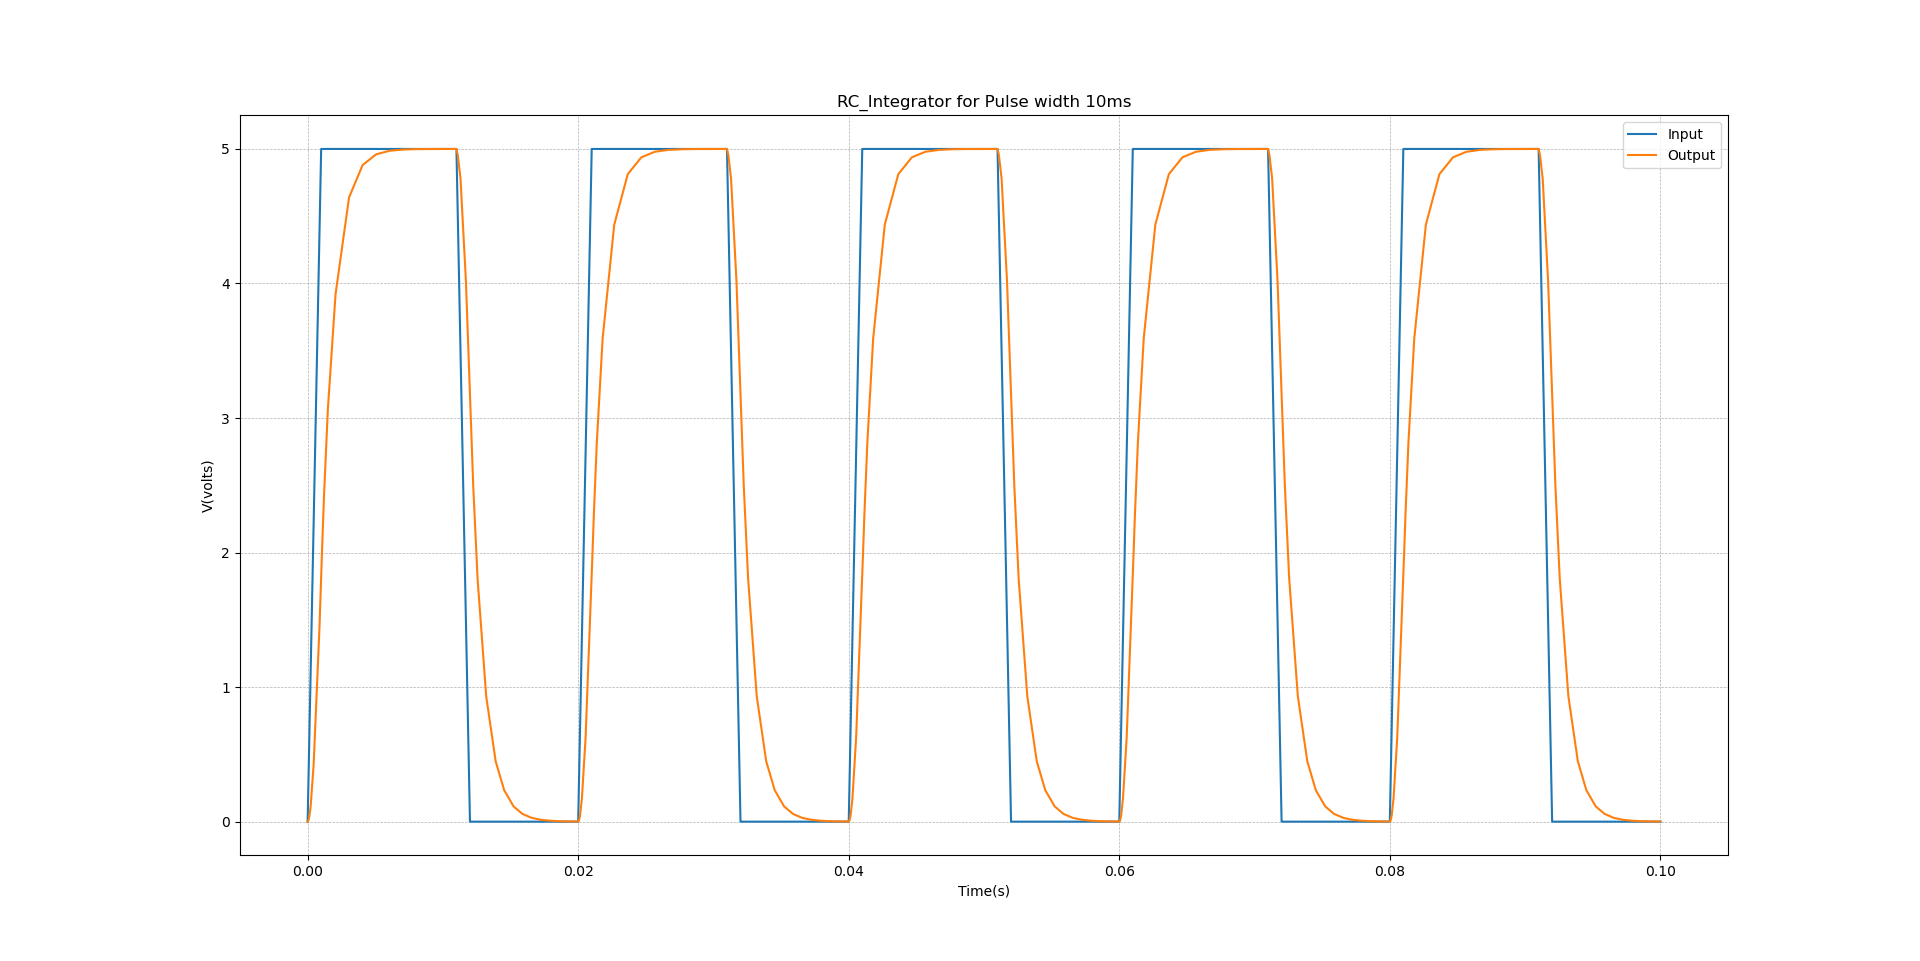
\includegraphics[width=\paperwidth]{RC_Integrator_1.png}}
\makebox[\textwidth]{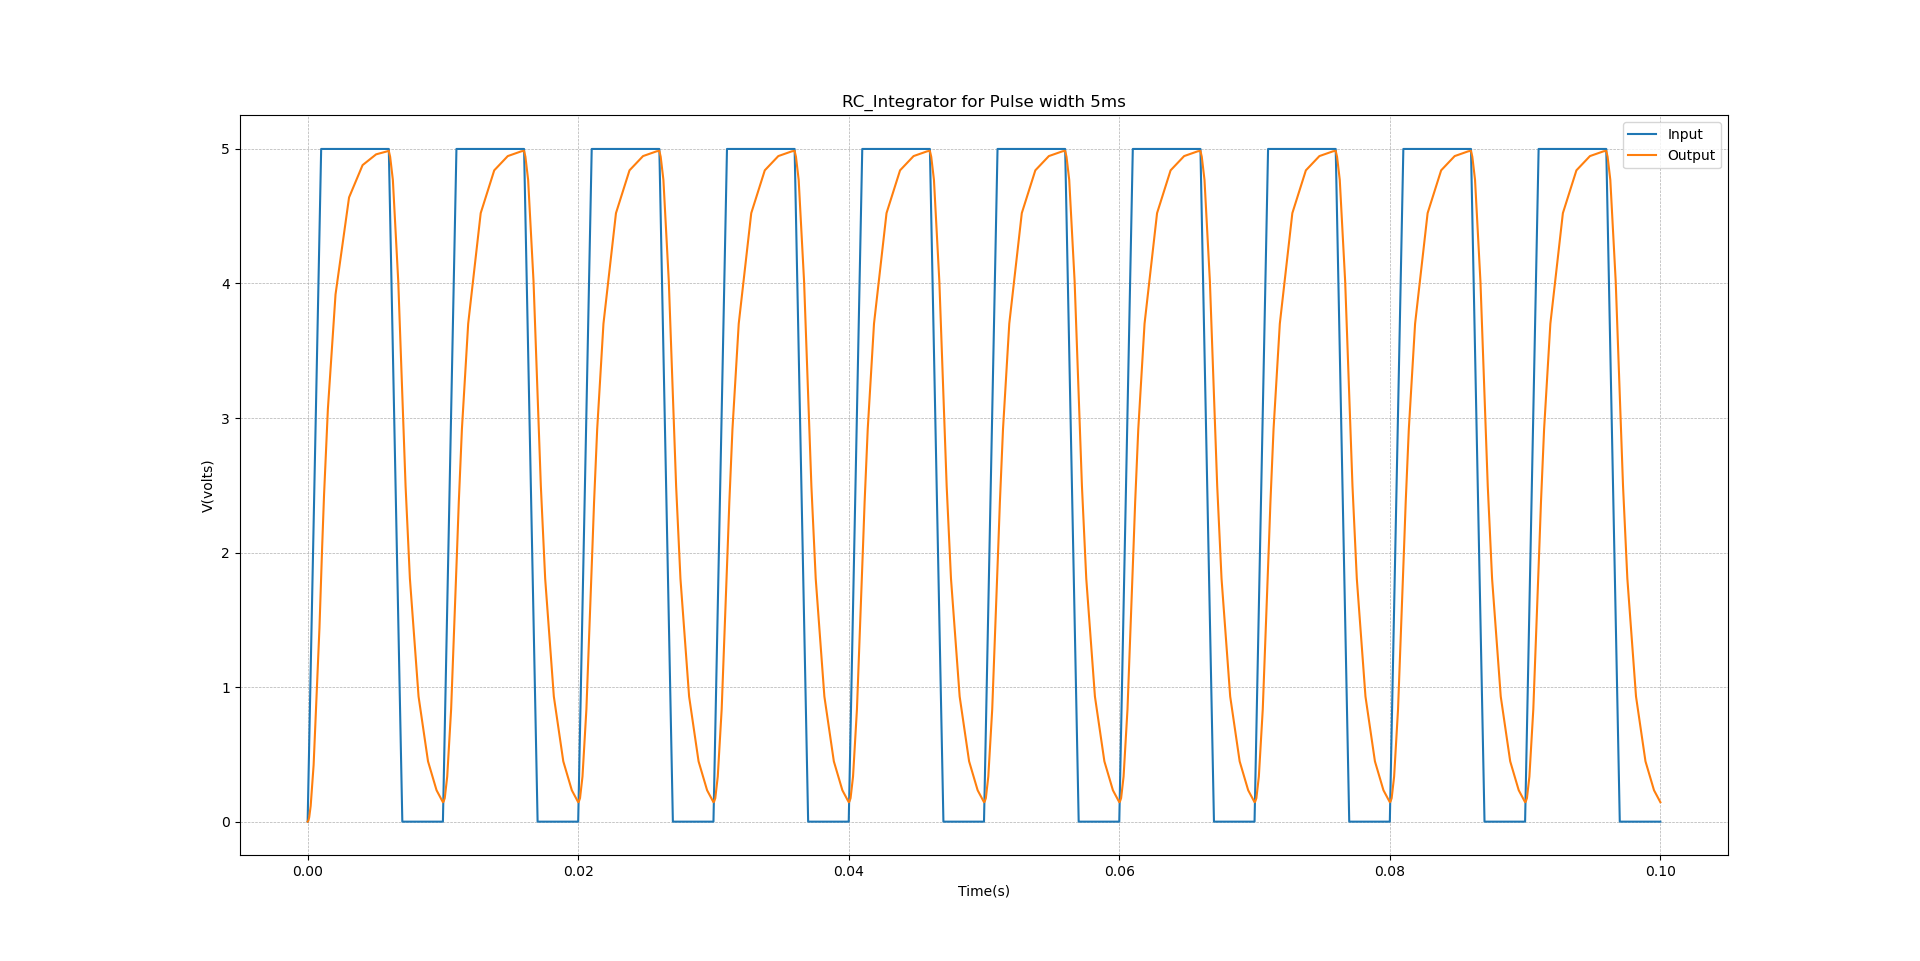
\includegraphics[width=\paperwidth]{RC_Integrator_2.png}}
\makebox[\textwidth]{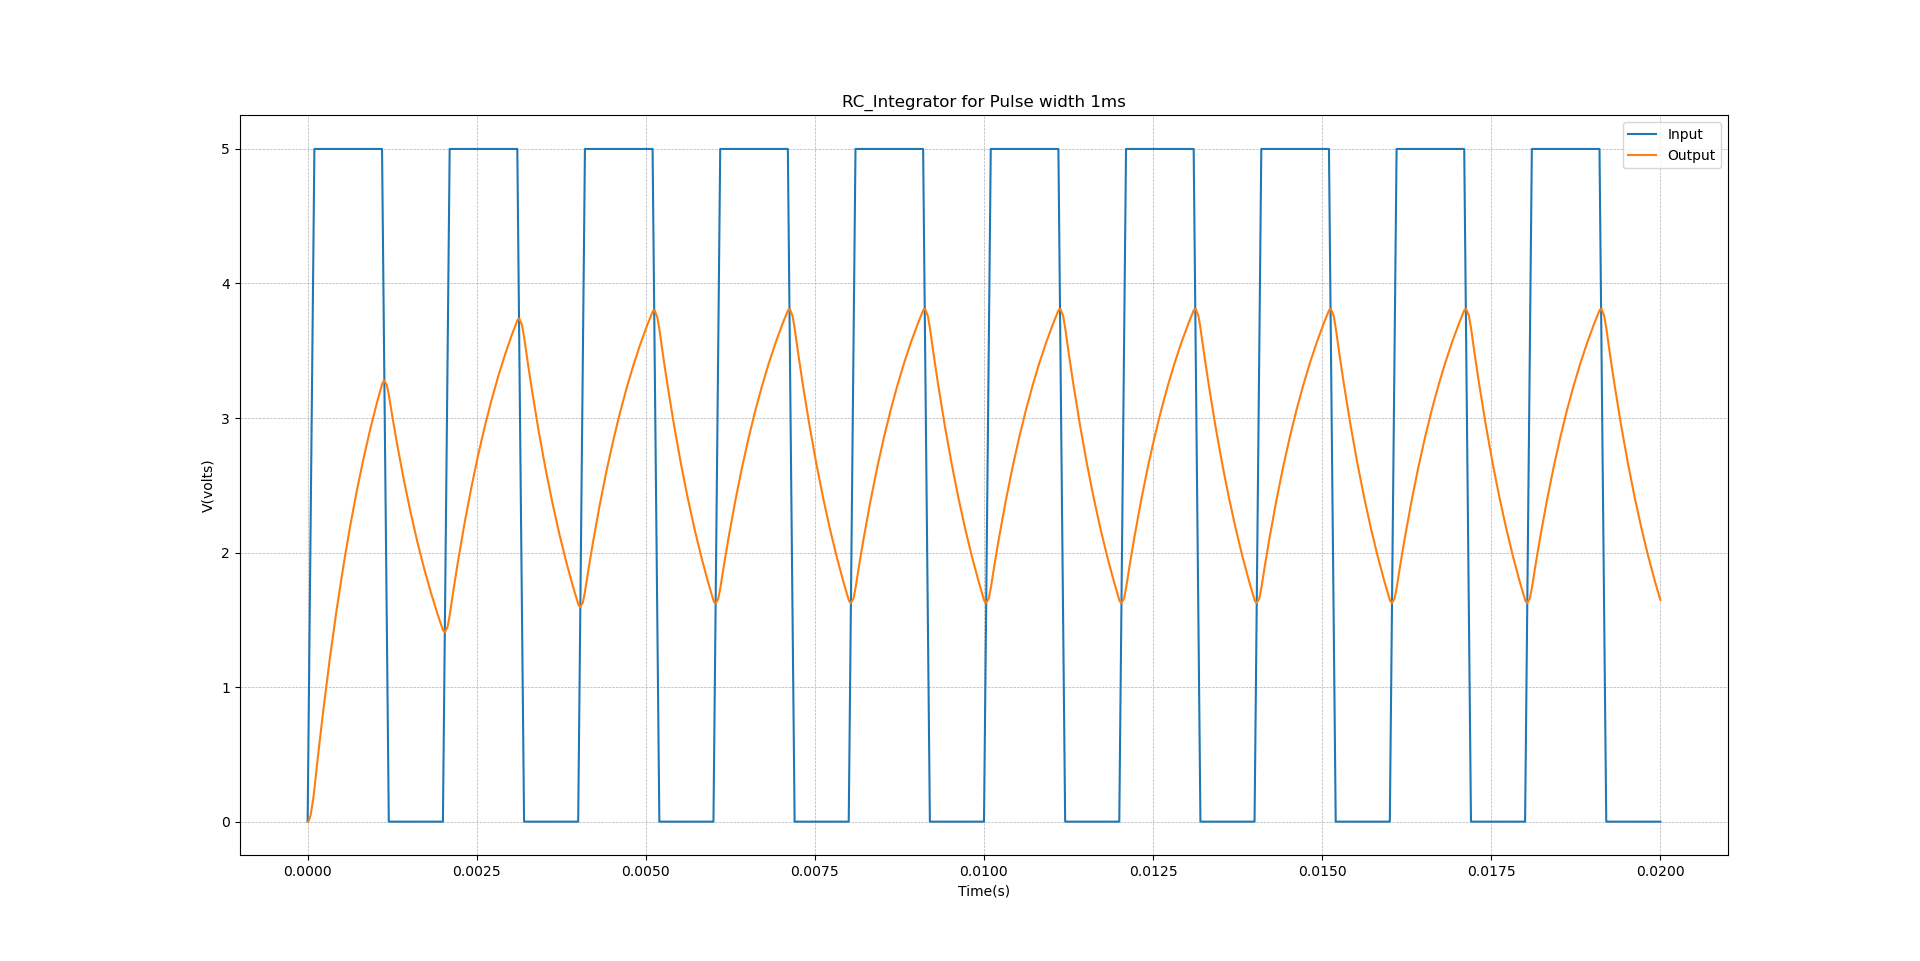
\includegraphics[width=\paperwidth]{RC_Integrator_3.png}}
\makebox[\textwidth]{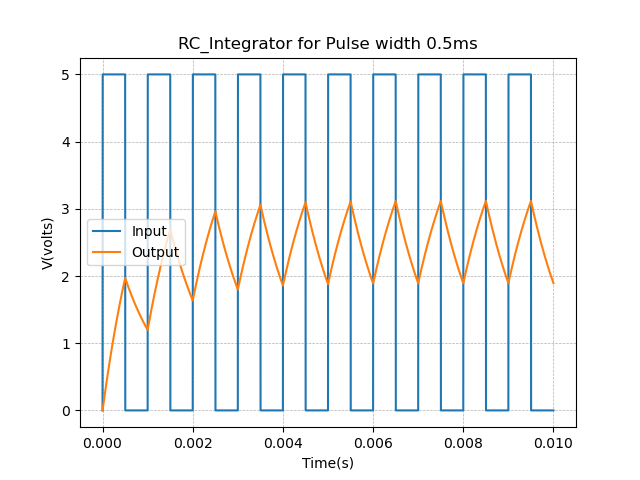
\includegraphics[width=\paperwidth]{RC_Integrator_4.png}}
\makebox[\textwidth]{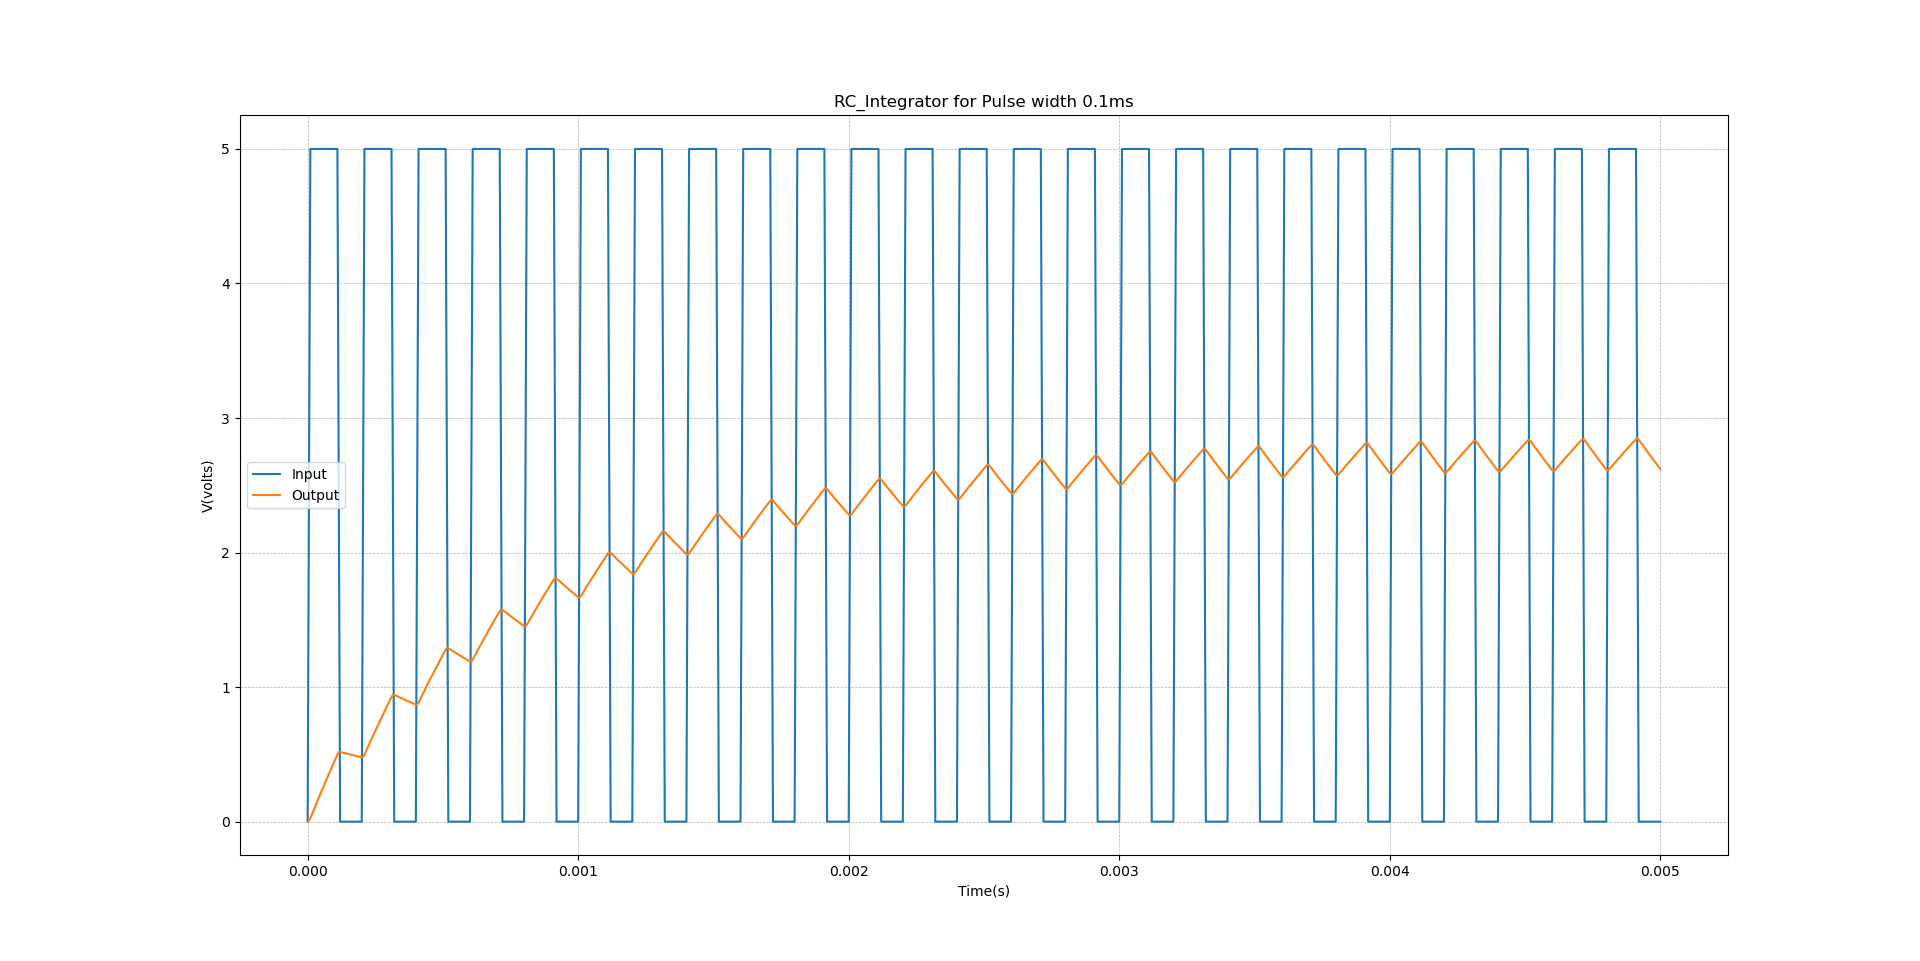
\includegraphics[width=\paperwidth]{RC_Integrator_5.png}}
\makebox[\textwidth]{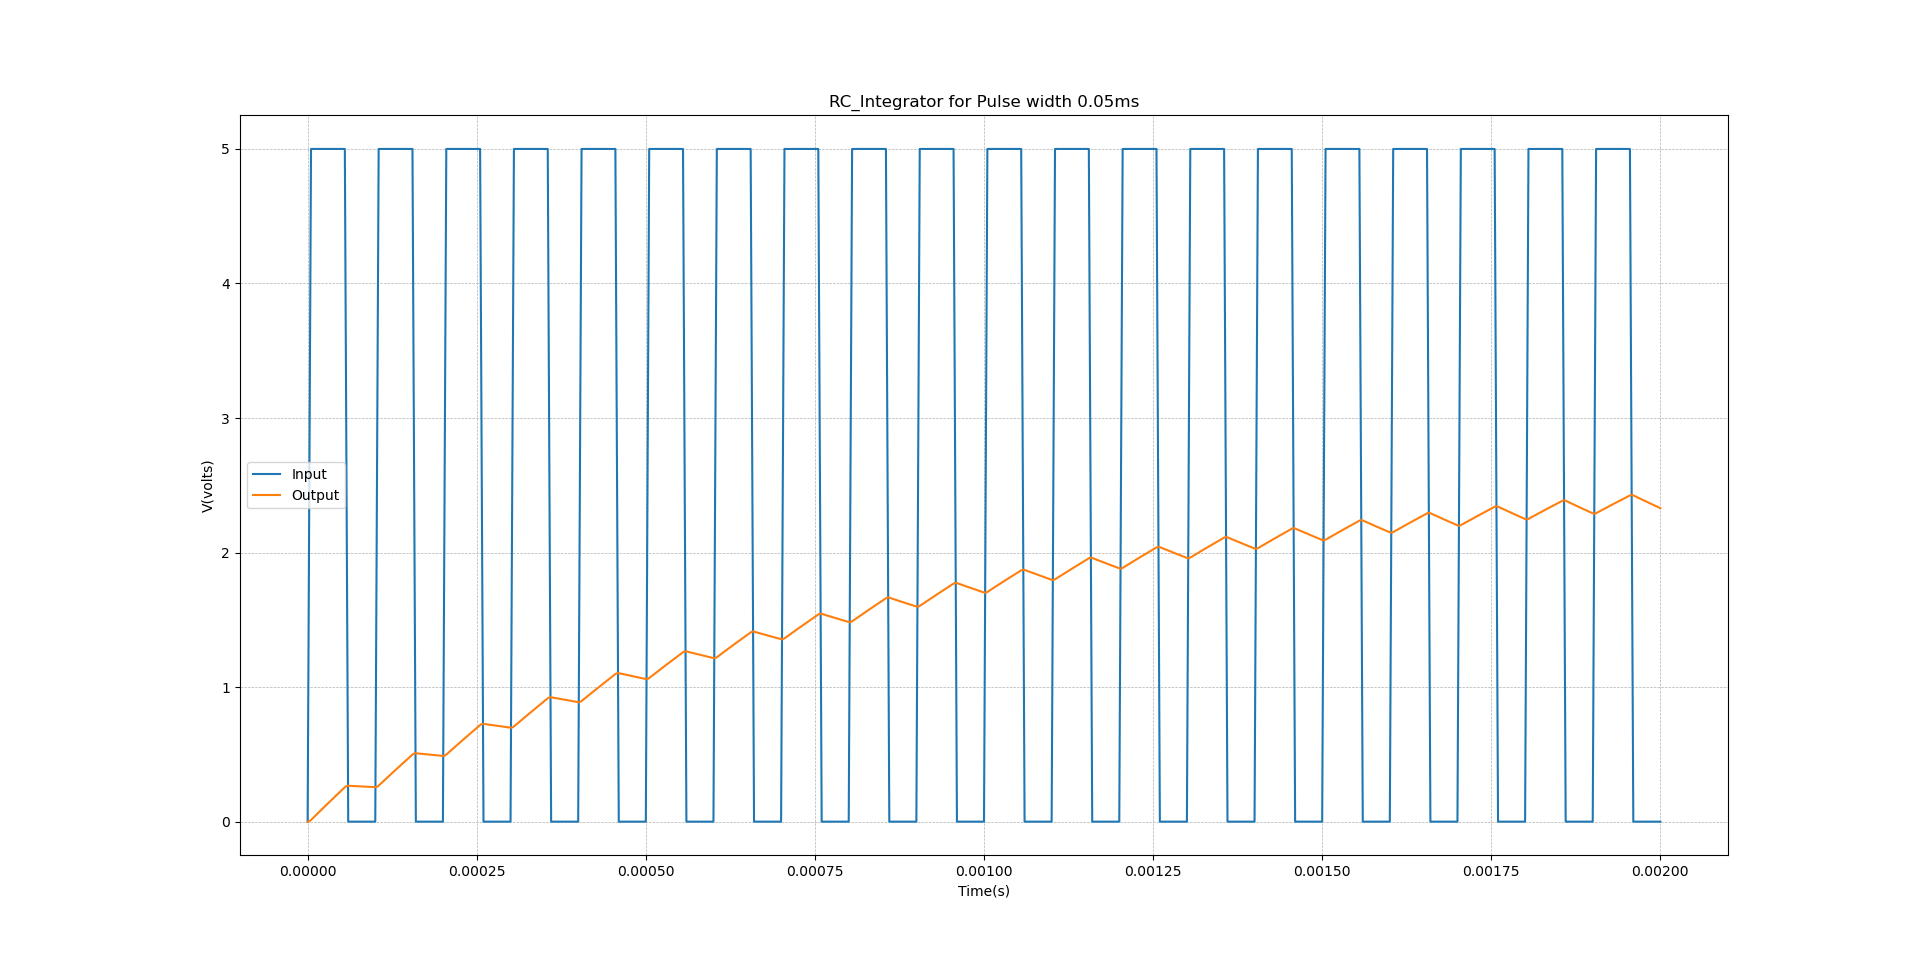
\includegraphics[width=\paperwidth]{RC_Integrator_6.png}}

\subsection{RC Differentiator}
\subsubsection{Code snippet}
\lstinputlisting[language=SPICE]{../RC_Differentiator.cir}
\subsubsection{Simulation results}
\makebox[\textwidth]{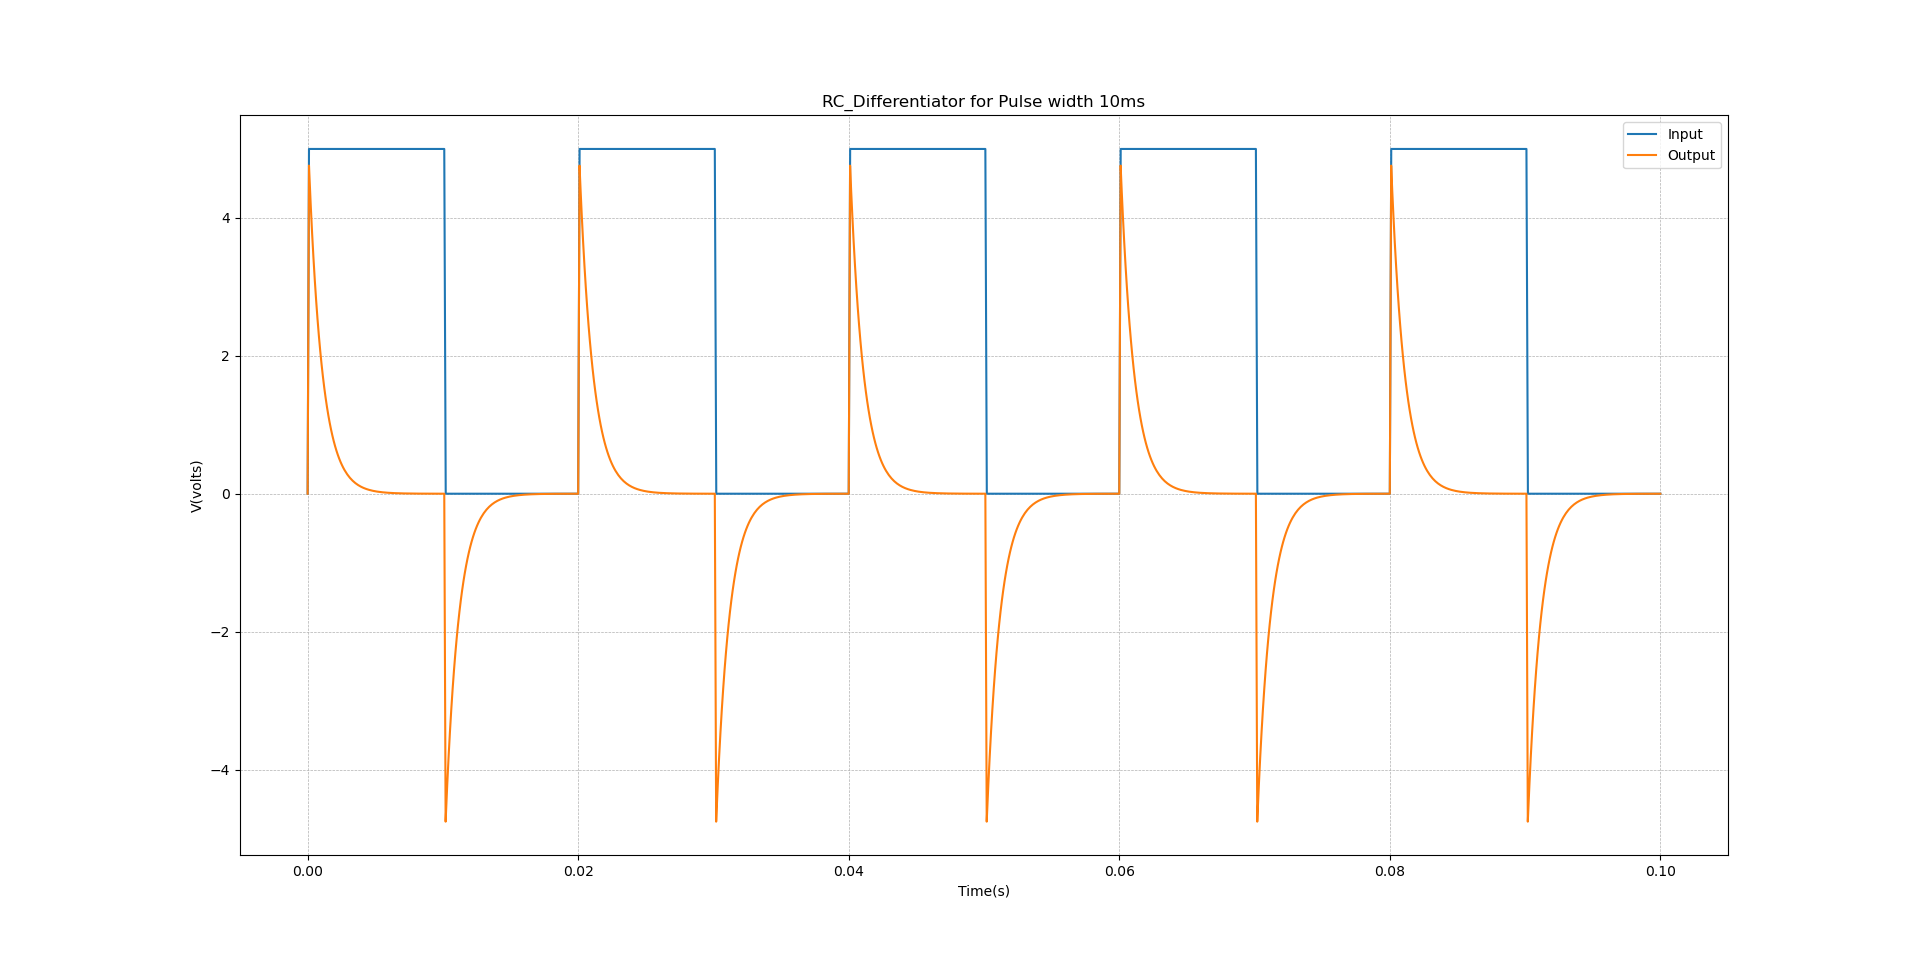
\includegraphics[width=\paperwidth]{RC_Differentiator_1.png}}
\makebox[\textwidth]{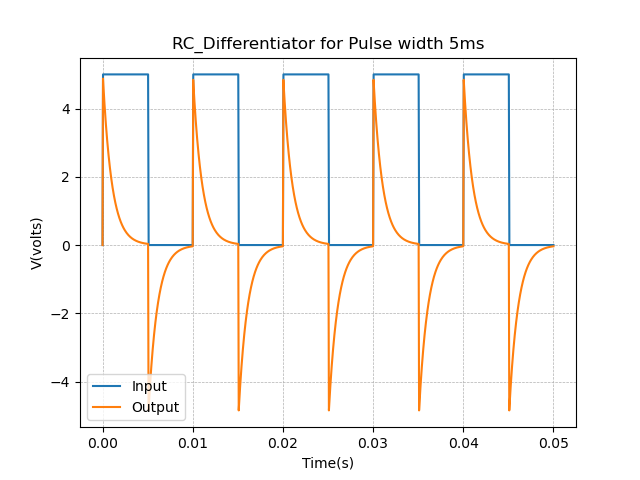
\includegraphics[width=\paperwidth]{RC_Differentiator_2.png}}
\makebox[\textwidth]{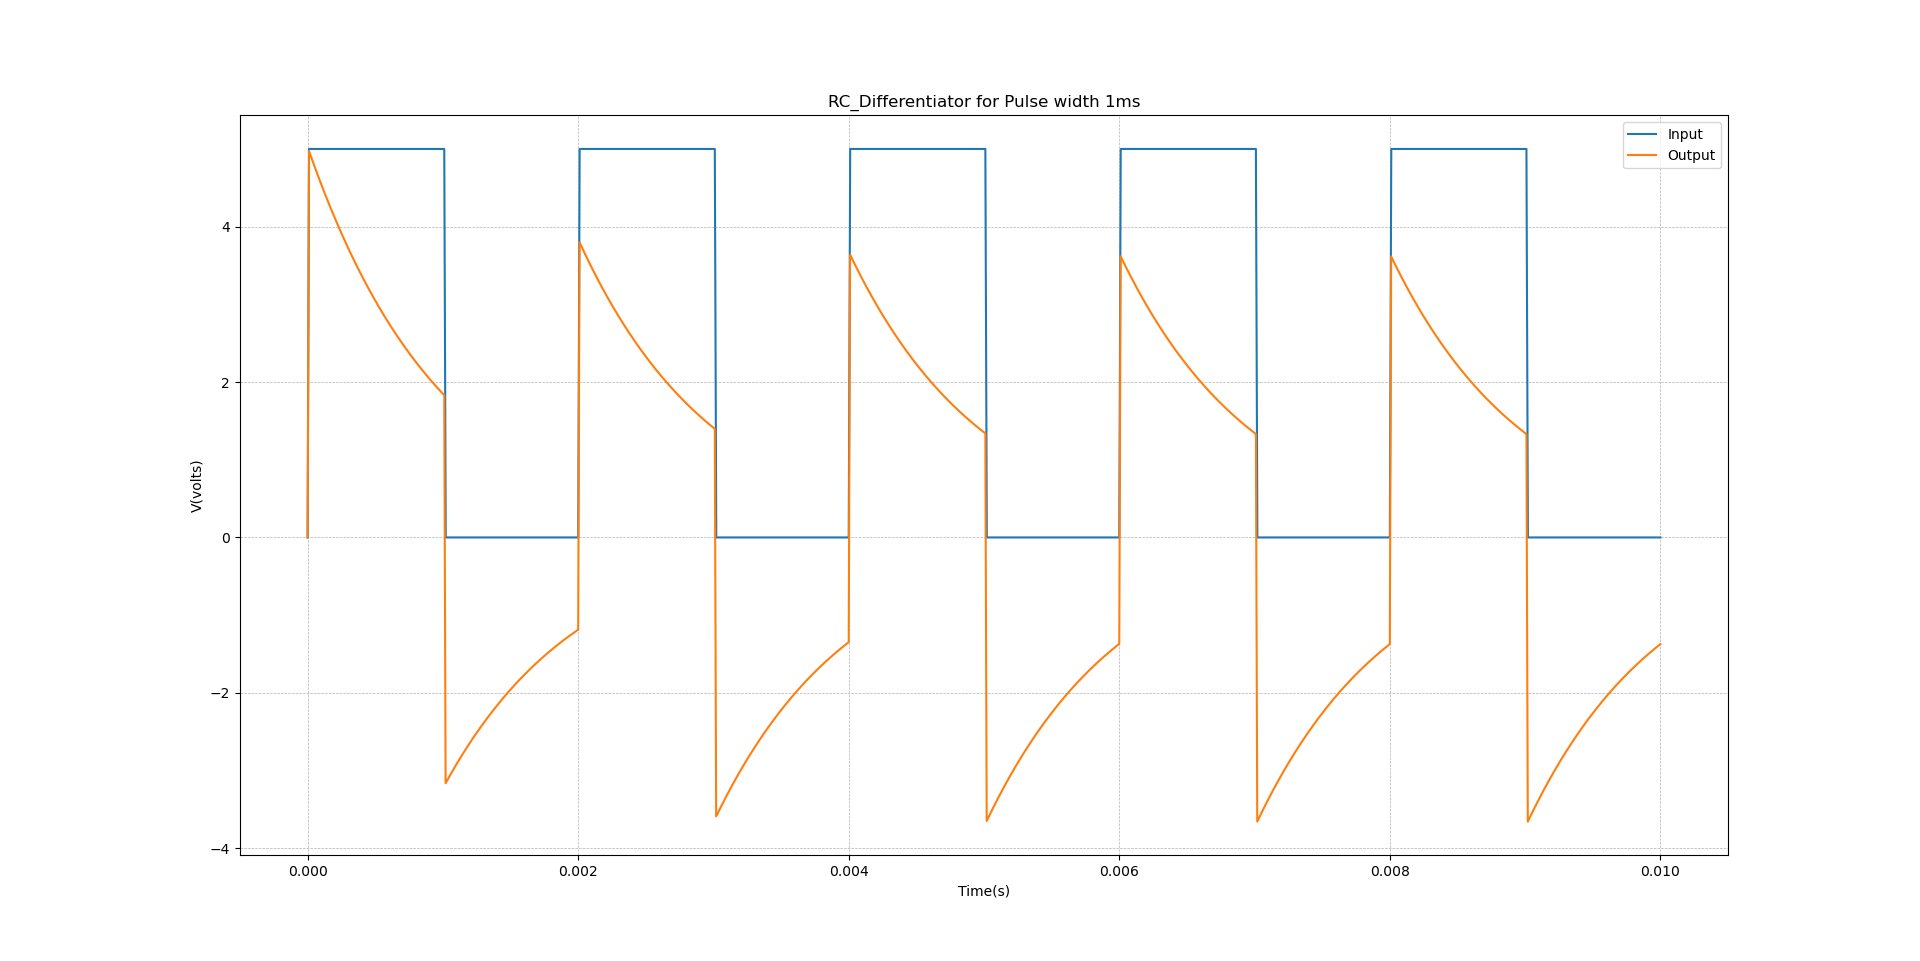
\includegraphics[width=\paperwidth]{RC_Differentiator_3.png}}
\makebox[\textwidth]{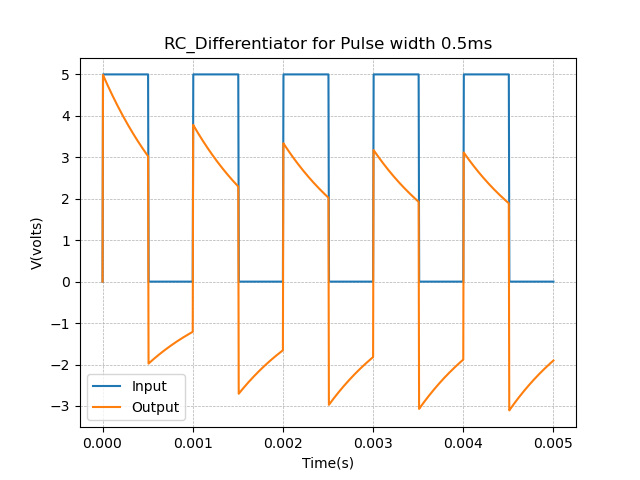
\includegraphics[width=\paperwidth]{RC_Differentiator_4.png}}
\makebox[\textwidth]{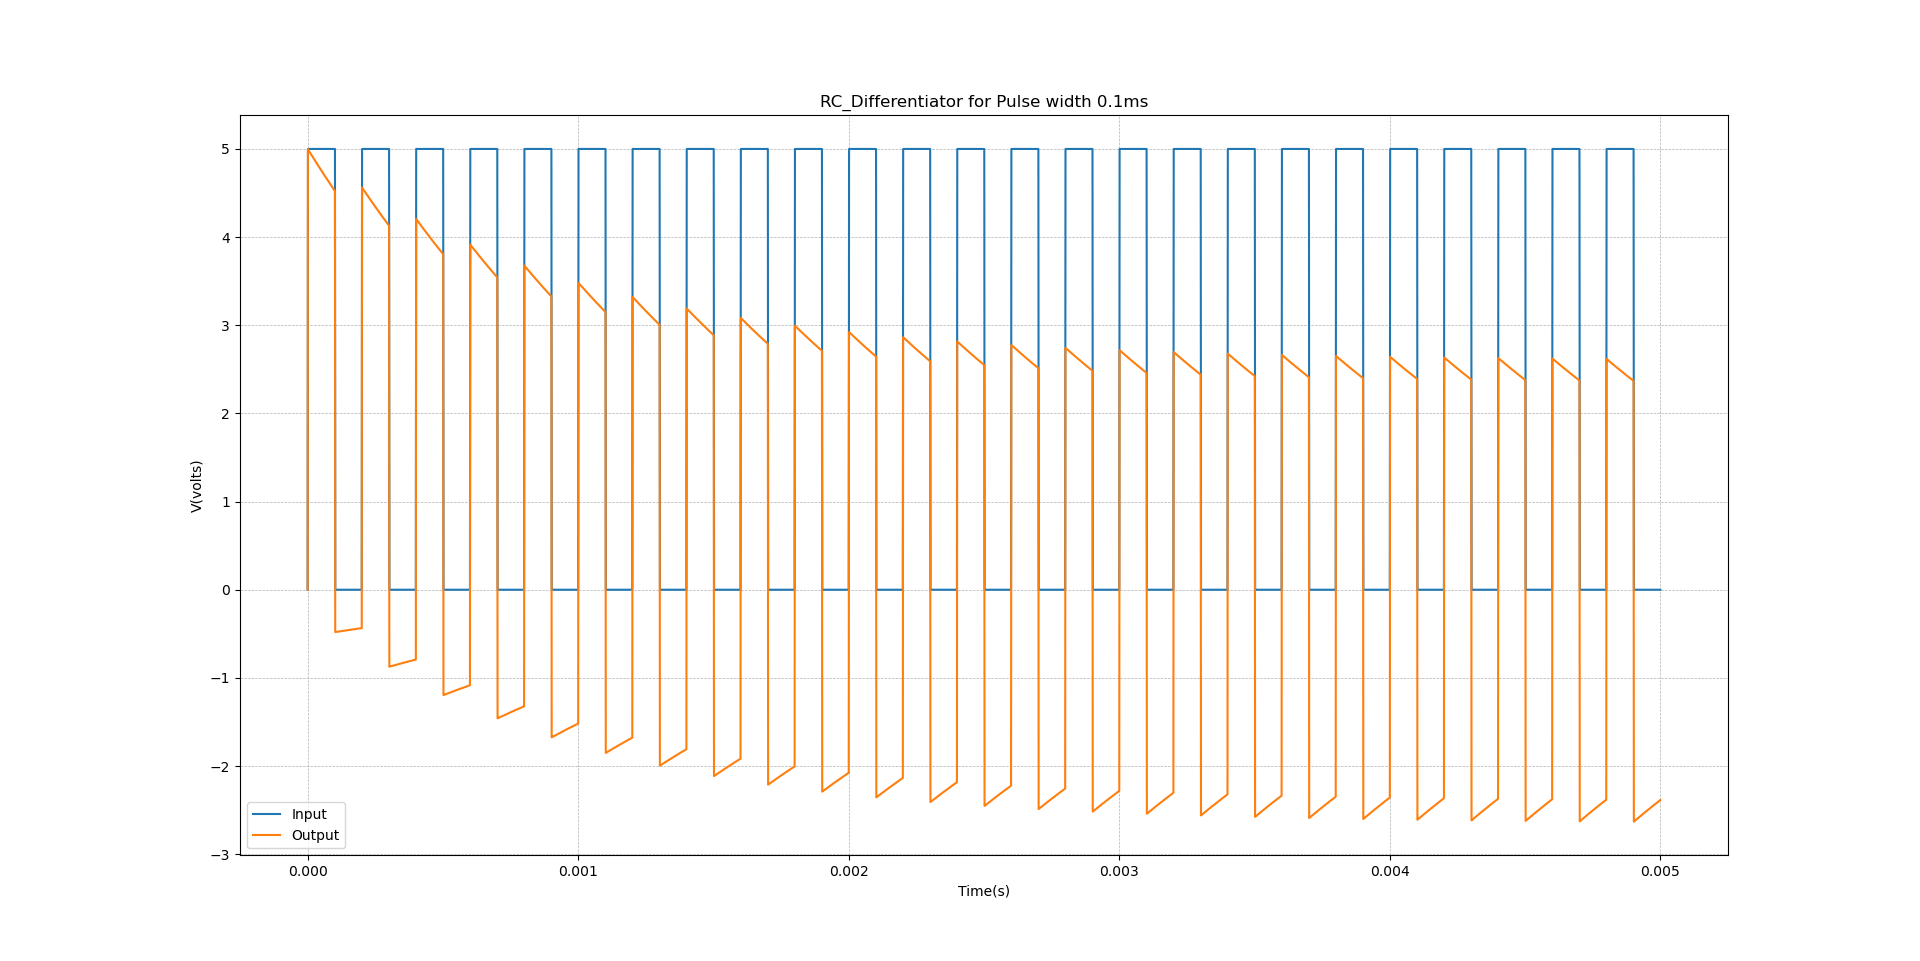
\includegraphics[width=\paperwidth]{RC_Differentiator_5.png}}
\makebox[\textwidth]{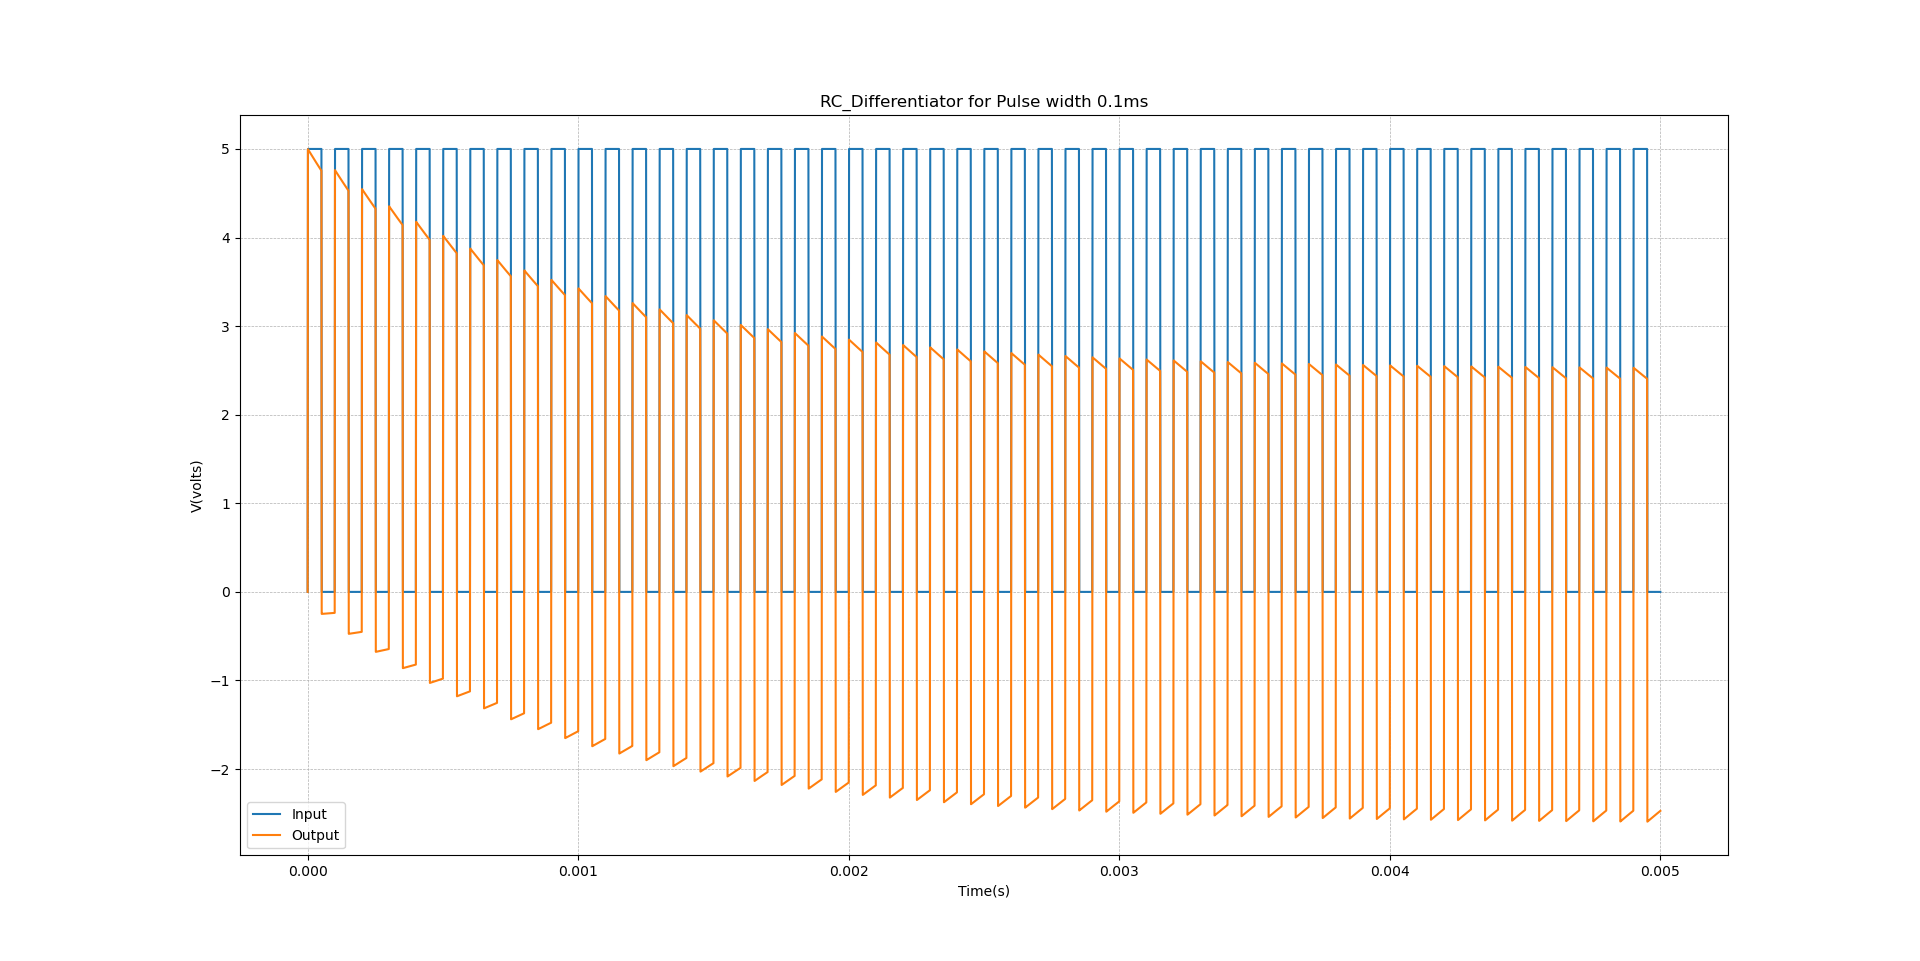
\includegraphics[width=\paperwidth]{RC_Differentiator_6.png}}

\subsection{RC Lowpass Filter}
\subsubsection{Code snippet}
\lstinputlisting[language=SPICE]{../RC_Lowpass_Filter.cir}
\subsubsection{Simulation results}
\makebox[\textwidth]{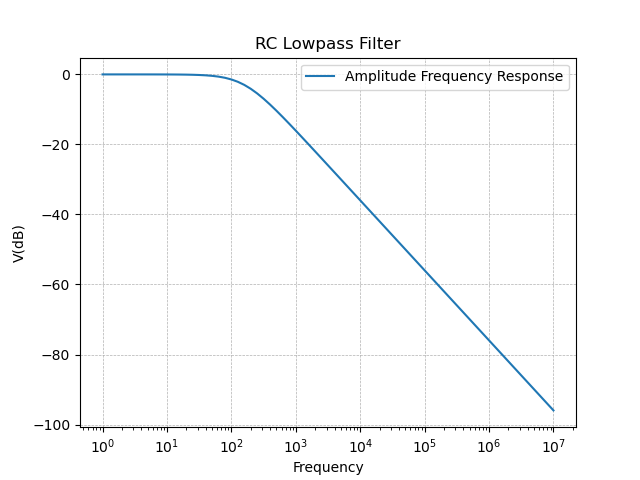
\includegraphics[width=\paperwidth]{RC_Lowpass_Filter.png}}

\subsection{RC Highpass Filter}
\subsubsection{Code snippet}
\lstinputlisting[language=SPICE]{../RC_Highpass_Filter.cir}
\subsubsection{Simulation results}
\makebox[\textwidth]{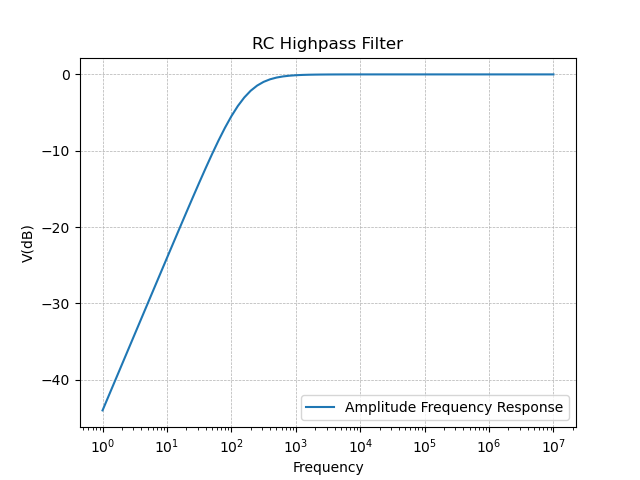
\includegraphics[width=\paperwidth]{RC_Highpass_Filter.png}}

\subsection{RC Bandpass Filter}
\subsubsection{Code snippet}
\lstinputlisting[language=SPICE]{../RC_Bandpass_Filter.cir}
\subsubsection{Simulation results}
\makebox[\textwidth]{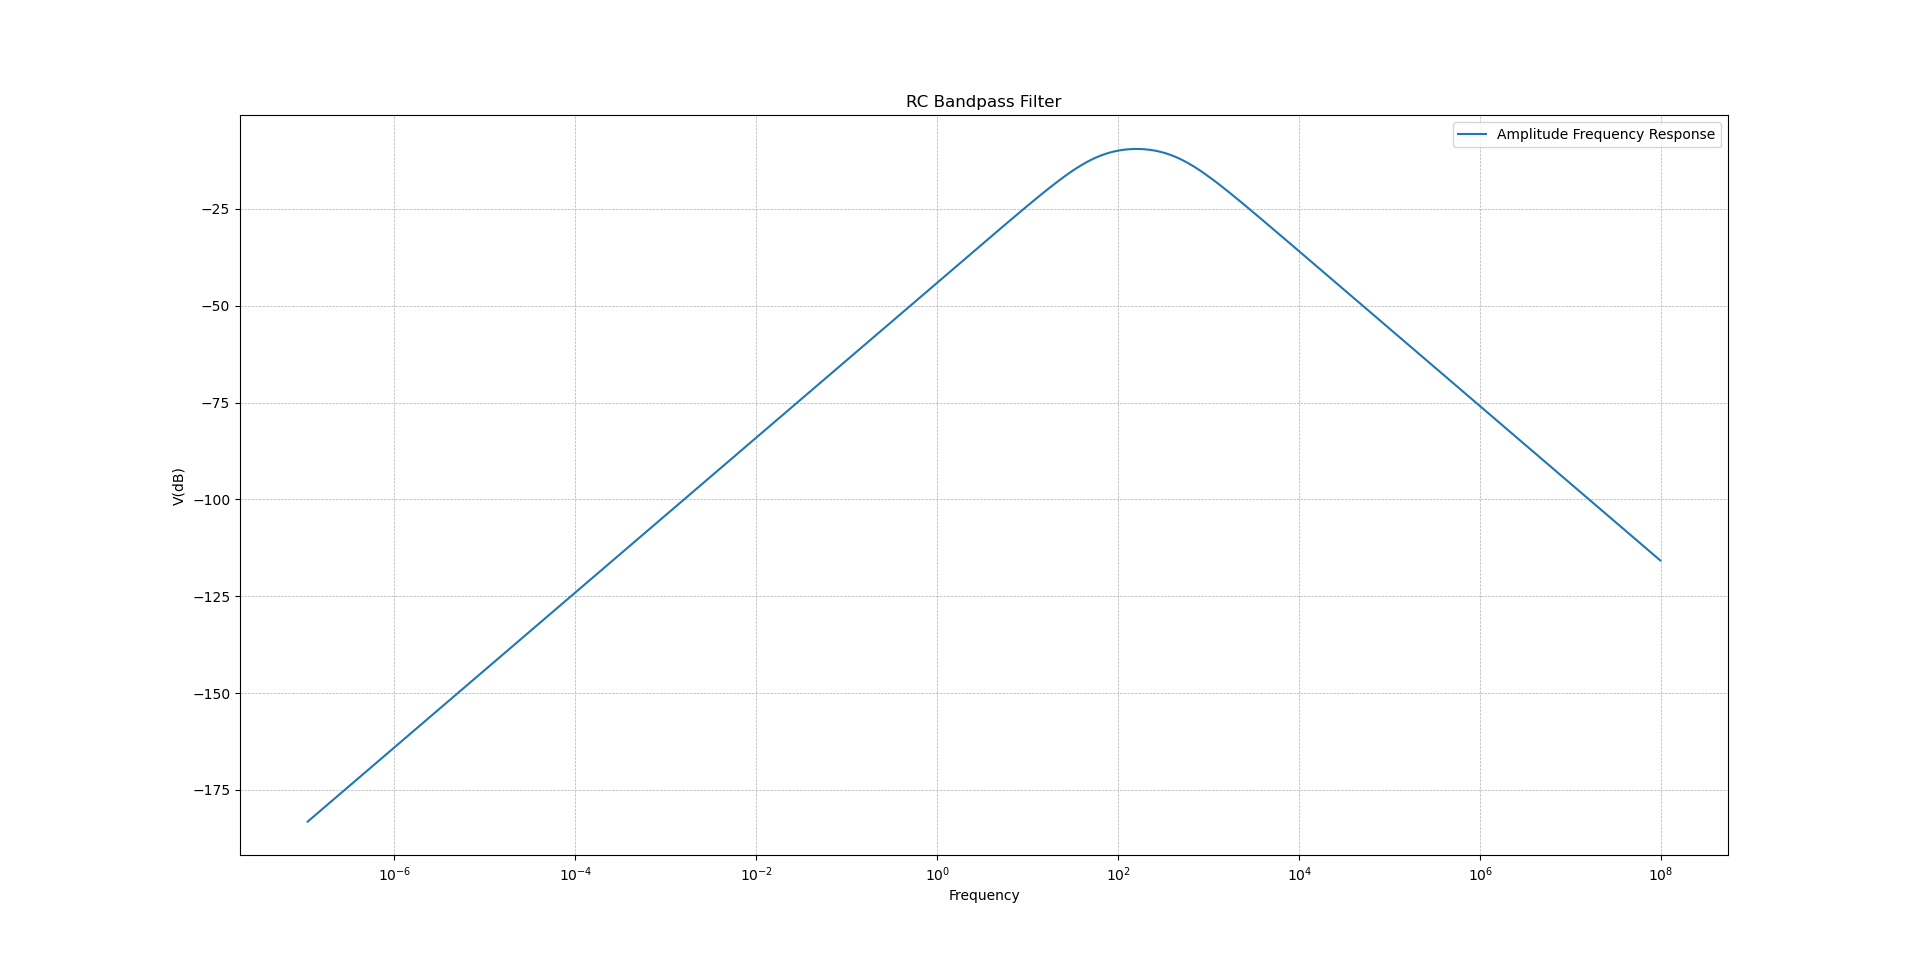
\includegraphics[width=\paperwidth]{RC_Bandpass_Filter.png}}

\subsection{RLC Bandpass Filter}
\subsubsection{Code snippet}
\lstinputlisting[language=SPICE]{../RLC_Bandpass_Filter.cir}
\subsubsection{Simulation results}
\makebox[\textwidth]{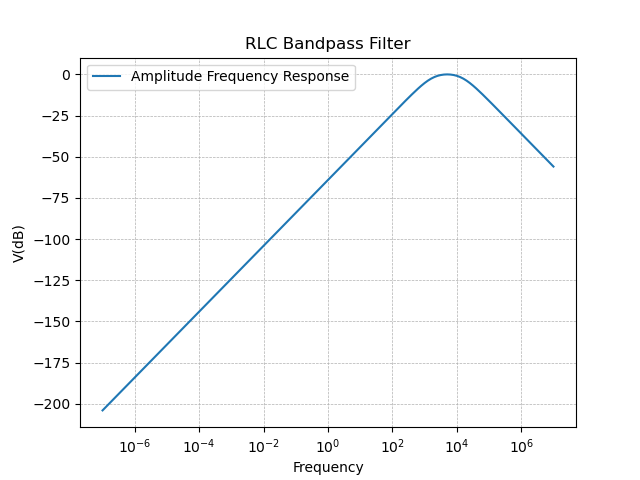
\includegraphics[width=\paperwidth]{RLC_Bandpass_FiIter.png}}


\section{Experimental results}

\subsection{RC Integrator}

$\tau= RC = 10K\Omega \cdot 0.1\mu F=1ms$ The circuit is simulated for 
pulsewidth $T$, where $T=\{10\tau,5\tau,\tau,0.5\tau,0.1\tau,0.01\tau\}$

\subsection{RC Differentiator}
$\tau= RC = 10K\Omega \cdot 0.1\mu F=1ms$ The circuit is simulated for 
pulsewidth $T$, where $T=\{10\tau,5\tau,\tau,0.5\tau,0.1\tau,0.01\tau\}$

\subsection{RC Lowpass Filter}
The Transfer Function is $$G(s)=\frac{1}{1+sRC}$$

The 3db frequency is expected to be $$f_{3db}=\frac{1}{2\pi}\cdot\frac{1}{RC}=159.16Hz$$
The experimental value follows it quite closely.
\subsection{RC Highpass Filter}
The Transfer Function is $$G(s)=\frac{sRC}{1+sRC}$$

The 3db frequency is expected to be $$f_{3db}=\frac{1}{2\pi}\cdot\frac{1}{RC}=159.16Hz$$ 
The experimental value follows it quite closely.

\subsection{RC Bandpass Filter}
The Transfer Function is $$G(s)=\frac{1}{3+sRC+\frac{1}{sRC}}$$

The peak frequency is expected to be $$f_{peak}=\frac{1}{2\pi}\cdot\frac{1}{RC}=159.16Hz$$ 
The lower and higher frequencies are expected to be 
$$f_{L}=\frac{\sqrt{13}-3}{2}\cdot\frac{1}{2\pi}\cdot\frac{1}{RC}=48.189Hz$$ 
$$f_{H}=\frac{\sqrt{13}+3}{2}\cdot\frac{1}{2\pi}\cdot\frac{1}{RC}=525.67Hz$$
The experimental values are 

$f_{L}=49.33Hz$,$f_{H}=532.9Hz$ with $f_{peak}=162.1Hz$ and peak amplitude = -9.5 db

They follow theoretical values follows it quite closely.
\subsection{RLC Bandpass Filter}
The Transfer Function is $$G(s)=\frac{R}{R+sC+\frac{1}{sL}}$$

The peak frequency is expected to be $$f_{peak}=\frac{1}{2\pi}\cdot\frac{1}{\sqrt{LC}}=5.032KHz$$ 
The lower and higher frequencies are expected to be 
$$f_{L}=\frac{1}{2\pi}\cdot\frac{\sqrt{(RC)^{2}+4LC}-RC}{2LC}=1.46KHz$$ 
$$f_{H}=\frac{1}{2\pi}\cdot\frac{\sqrt{(RC)^{2}+4LC}+RC}{2LC}=17.37KHz$$
The experimental values are 

$f_{L}=1.448Hz$,$f_{H}=17.339Hz$ with $f_{peak}=5.035KHz$.

They follow theoretical values follows it quite closely.

\section{Experiment completion status}
All the sections were completed
\end{document}
